\begin{theorem}
    Sea $D\in\Re^2$ una regi\'on simplemente conexa (o tipo 3) y sea $\partial D$ la frontera de $D$, con orientaci\'on tal que se cumple la regla de la mano derecha. Sea $\mathbf{F}:D\to\Re^2$ de clase $C^1$. Entonces
    \[
        \oint_{\partial D}\mathbf{F}\cdot d\mathbf{s} = \iint_D \nabla\times\mathbf{F}\cdot d\mathbf{A}
    \]
\end{theorem}

Otra manera de enunciar el teorema de Green es usando un cambio en la notaci\'on vectorial. Pensando el producto escalar $\mathbf{F}\cdot d\mathbf{s}$ como $P\:dx+Q\:dy$, donde $\mathbf{F}=(P,Q)$ y sabiendo que el rotor en $\Re^2$ es la componente $z$ del rotor en $\Re^3$; reescribimos el teorema de Green como
\[
        \int_{C^+}P\:dx+Q\:dy=\int_D\left(\frac{\partial Q}{\partial x}-\frac{\partial P}{\partial y}\right).
\]

El teorema de Green es aplicable a regiones a\'un m\'as generales que simplemente conexas. De hecho, a cualquier regi\'on en $\Re^2$ cuya frontera se pueda descomponer en un n\'umero finito de curvas cerradas simples orientadas se le puede aplicar el teorema de Green. La idea es ``recorrer" dicha frontera pasando por todas las curvas que la confroman.

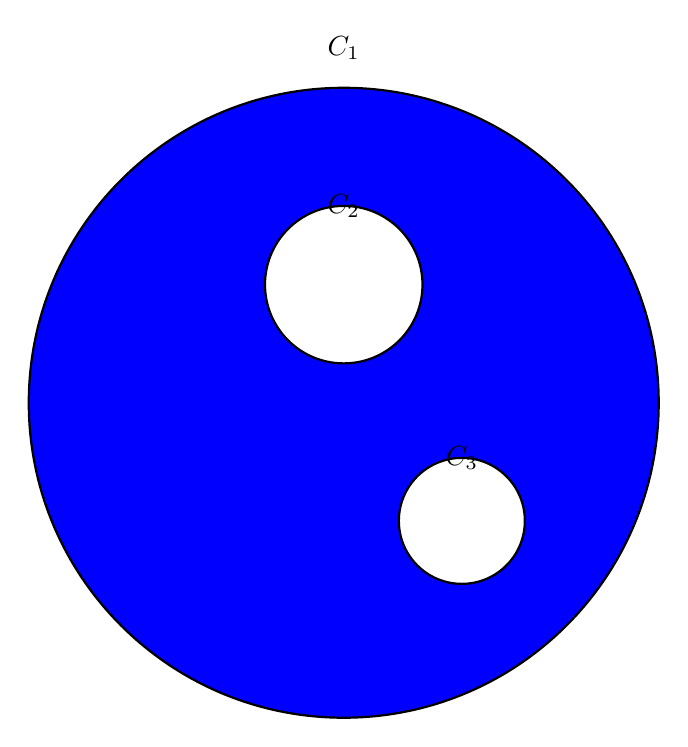
\begin{tikzpicture}
    % Define the exterior boundary
    \draw[thick, fill=blue] (0,0) circle (4);

    % Define the inner boundaries
    \draw[thick, fill=white] (0,1.5) circle (1);
    \draw[thick, fill=white] (1.5,-1.5) circle (0.8);

    % % Draw arrows for the outer boundary
    % \draw[thick,->] (0,4) arc (90:45:4);
    % \draw[thick,->] (4,0) arc (0:-45:4);
    % \draw[thick,->] (0,-4) arc (270:225:4);
    % \draw[thick,->] (-4,0) arc (180:135:4);

    % % Draw arrows for the inner boundaries (clockwise direction)
    % \draw[thick,->] (0,2.5) arc (90:45:1);
    % \draw[thick,->] (1.5,-0.7) arc (90:45:0.8);

    % Label the regions
    \node at (0,4.5) {$C_1$};
    \node at (0,2.5) {$C_2$};
    \node at (1.5,-0.7) {$C_3$};

\end{tikzpicture}
